\scanpage{73}\mspage{72}

sous-figure de \deleted{$\unsure{G'|F'}$} la subdivision $F'$ de $F$, induite par la sous-figure $\deleted{F}G$ de $F$.
% slanted; three short oblique lines, with de low at the left of the last line.
\margin{double Transitivité de l'induction}

$\uline{C}7_0$ Pour toute figure $F$, sous-figure $G$, et subdivision $G'$ de $G$, il existe une subdivision $F'$ de $F$ qui induise $\unsure{C'|G'}$,

(mais l'énoncé symétrique, où on échangerait les \unsure{rôle|rôles} de
% fig:order-overlap. The upper arm belongs to / meets the q descender above;
% the short worked group does not establish a separate complete deleted letter.
\unsure{\begin{tikzpicture}[x=1ex,y=1ex,baseline=-.25ex,line width=.45pt]
\draw (.30,1.55) .. controls (.48,1.05) and (.55,.25) .. (.38,-.15) -- (.57,-.17);
\draw (.12,.62) -- (.17,.02) -- (.59,.72);
\draw (.16,.27) -- (.55,.53);
\end{tikzpicture}}
$\leq$ et $\preceq$, est faux
% fig:faux-mark. Curled worked sign and its two crossing arms; colon is separate.
\unsure{\begin{tikzpicture}[x=1ex,y=1ex,baseline=-.3ex,line width=.45pt]
\draw (.46,1.27) .. controls (.36,1.52) and (.08,1.03) .. (.14,.70)
 .. controls (.10,.40) and (.49,.28) .. (.43,.10)
 .. controls (.43,-.04) and (.30,-.29) .. (.27,-.43);
\draw (.06,1.24) .. controls (.15,.89) and (.21,.50) .. (.34,.24);
\draw (.06,.65) -- (.79,1.33);
\draw (-.03,.94) -- (.23,.85);
\end{tikzpicture}}
: il n'est pas vrai, pour $F'\preceq F$ \unsure{donnés|données}, que tte sous figure $G'$ de $F'$ \unsure{soit|sont|est} induite par une ss-figure $G$ de $\deleted{G}F$).

On \deleted{peut} \unsure{renforcera|renforce} par la suite $C7_0$ en
% fig:before-C7. One separate low curved stroke, with no secure crossing stroke.
\unsure{\begin{tikzpicture}[x=1ex,y=1ex,baseline=-.25ex,line width=.45pt]
\draw (0,0) .. controls (.24,.10) and (.37,.38) .. (.35,.62);
\end{tikzpicture}}$C7$, en prenant un choix canonique de $F'$.

% fig:cancelled-draft. The text appears once. Actual local and broad cancellation
% strokes are drawn, rather than adding synthetic horizontal strikes to each line.
% The last line is below all three broad stroke endpoints: its cancellation state,
% not its lettering, is the doubt attached to that line.
\figure{\begin{tikzpicture}[x=.01cm,y=-.01cm,line width=.5pt,
  every node/.style={font=\small,inner sep=0pt}]
\path[use as bounding box] (0,0) rectangle (1400,900);
\node[anchor=west] at (32,102) {\unsure{Corollaire|Comparabilité} \unsure{1}};
% Local scribble over the title, and its shorter underline.
\draw (80,70) -- (71,134) -- (112,74) -- (92,139) -- (142,84)
 -- (125,150) .. controls (144,159) and (166,130) .. (181,110)
 -- (213,139) -- (204,65) -- (233,143) -- (285,88)
 .. controls (295,88) and (275,142) .. (285,145)
 -- (353,83) .. controls (360,98) and (335,124) .. (352,133)
 -- (396,74);
\draw (35,160) -- (350,154);
\node[anchor=west] at (560,100) {Soient $F,\deleted{A}G$ deux figures.};

\node[anchor=west] at (25,188) {\inserted{Considérons les}};
% fig:insertion-enclosure. Right upturn and descending left connector retained.
\draw (30,255) .. controls (15,225) and (39,213) .. (65,205)
 .. controls (175,194) and (330,199) .. (400,180)
 .. controls (420,176) and (418,160) .. (411,151);
\node[anchor=west] at (28,234) {Conditions \deleted{équivalentes} :};

\node[anchor=west] at (125,307) {a) $G$ est une sous-figure d'une subd. de $F$ :};
\node[anchor=west] at (450,397) {\begin{minipage}{4cm}\[G\leq F'\preceq F\]\end{minipage}};
\node[anchor=north west,text width=12cm,align=left] at (118,460) {b) $G$ est une subdivision d'une sous-figure de $F$ :};
\node[anchor=west] at (417,625) {\begin{minipage}{4cm}\[G\preceq G'\leq F.\]\end{minipage}};

\node[anchor=west,rotate=3] at (90,700) {On a alors b) $\Rightarrow$ a)};
\node[anchor=west,rotate=3] at (705,663) {(Mais pas \unsure{vrai|vice}\unsure{,} a $\Rightarrow$ b !!!\unsure{\begin{tikzpicture}[x=1ex,y=1ex,baseline=-.4ex,line width=.45pt]
% fig:draft-close-mark. Closing curve with a short right tick at mid-height.
\draw (.05,1.65) .. controls (.74,1.34) and (.76,.02) .. (.05,-.27);
\draw (.55,.70) -- (.68,.77);
\end{tikzpicture}}};

\node[anchor=west,rotate=2.7] at (85,781) {a) $\Rightarrow$ b) résulte de $C6$};
\draw (90,771) -- (800,738);
\node[anchor=west] at (87,829) {\unsure{b) $\Longrightarrow$ a) résulte de $C7_0$}};

% fig:small-square. Literal worked relation, rounded left sign, lower dots,
% retraced lower G, and irregular dotted downward endpoint are retained.
\node[anchor=center] at (1120,751) {\begin{minipage}{2.85cm}
\diagram{\begin{tikzcd}[ampersand replacement=\&,column sep=2.2em,row sep=1.7em]
F \arrow[r,phantom,"{\unsure{
\begin{tikzpicture}[x=1ex,y=1ex,baseline=-.3ex,line width=.55pt]
\draw (0,.35) -- (.95,1.03);
\draw (0,.28) .. controls (.73,.37) and (1.28,.31) .. (1.53,-.15);
\draw (.08,-.13) .. controls (.72,-.10) and (1.04,-.17) .. (1.42,-.45);
\draw (.04,.29) .. controls (.77,.11) and (1.35,.66) .. (1.30,1.55);
\draw (.87,.32) .. controls (1.28,.45) and (1.48,.74) .. (1.62,1.19);
\end{tikzpicture}}}" description]
\arrow[d,phantom,"{\unsure{\cup|U}}" description]
\& F' \arrow[d,phantom,"{\begin{tikzpicture}[x=1ex,y=1ex,baseline=-.4ex,line width=.5pt]
\draw (0,1.45) .. controls (.13,1.32) and (.10,1.18) .. (.04,1.05);
\fill (-.02,.75) circle (.07);
\fill (.09,.65) circle (.07);
\fill (.05,.51) circle (.06);
\draw (-.28,.24) -- (.02,-.02) -- (.28,.18) .. controls (.30,.45) and (.18,.45) .. (.15,.32);
\draw (-.25,.29) .. controls (-.03,.48) and (.12,.38) .. (.20,.39);
\draw (-.21,.21) -- (.18,.23);
\end{tikzpicture}}" description] \\
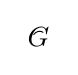
\begin{tikzpicture}[x=1ex,y=1ex,baseline=-.4ex]
\node[inner sep=0pt] at (0,0) {$G$};
\draw[line width=.35pt] (-.42,.20) .. controls (-.22,.52) and (.16,.55) .. (.40,.40);
\end{tikzpicture}
\arrow[r,phantom,"{\cdots}" description] \& G'
\end{tikzcd}}
\end{minipage}};

% Three broad cancellation strokes; the third is shorter than the other two.
\draw (180,100) -- (510,765);
\draw (757,38) -- (1143,784);
\draw (1119,38) -- (1310,370);
\end{tikzpicture}}
